\begin{surferPage}{Кејлијева кубна површ}
   Кубне површи  (површи трећег степена) су такође представљене 
    у галерији једноставних површи. 
    Све заједно кубна површ има 4 сингуларитета двоструке купе. Добила је има по 
	Артуру Кејлију, који је истраживао овакве површи у 19. веку.
    
    Међутим, први је 1863. године Лудвиг Шлефли направио систематску класификацију 
	ових површи на основу могућих сингуларитета.
    На пример, у његовом чланку се може прочитати зашто не може бити више од 4 
	сингуларне тачке на кубној површи.
    Ово доводи до: $\mu(3)=4$. 
    
    Око 1900. године Феликс Клајн је проучавао могуће облике реалних кубних површи. 
    Његова идеја била је да одговори на ово питање тако што би почео од Кејлијеве 
    површи уносећи мале деформације:
    ширећи сингуларитете двоструке купе или прекидајући или спајајући делове,
    он је успео да пронађе све могуће облике. Овде су неки од њих: 
    \vspace{0.3cm}
     \begin{center}
      \vspace{-0.2cm}
      \begin{tabular}{@{}c@{\ }c@{\ }c@{\ }c@{}}
        \begin{tabular}{@{}c@{}}
          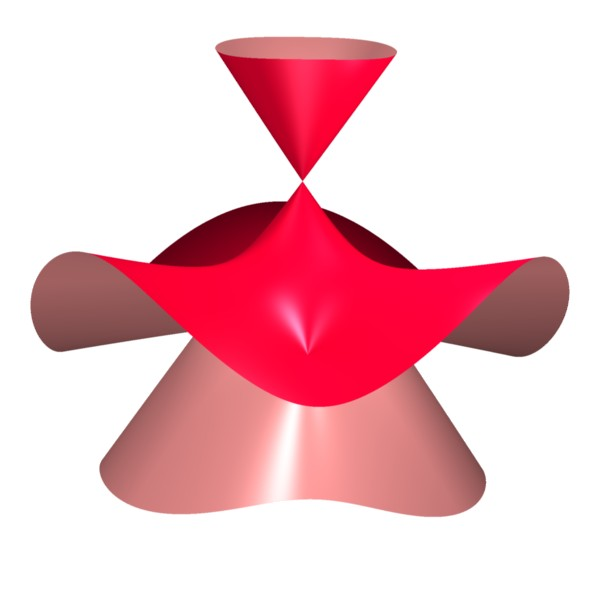
\includegraphics[width=1.35cm]{./../../common/images/cayley_cubic_0}
        \end{tabular}
        &
        \begin{tabular}{@{}c@{}}
          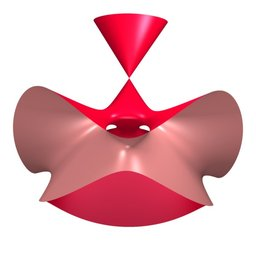
\includegraphics[width=1.35cm]{./../../common/images/cayley_cubic_1}
        \end{tabular}
        &
        \begin{tabular}{@{}c@{}}
          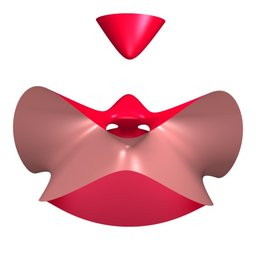
\includegraphics[width=1.35cm]{./../../common/images/cayley_cubic_2}
        \end{tabular}
        &
        \begin{tabular}{@{}c@{}}
          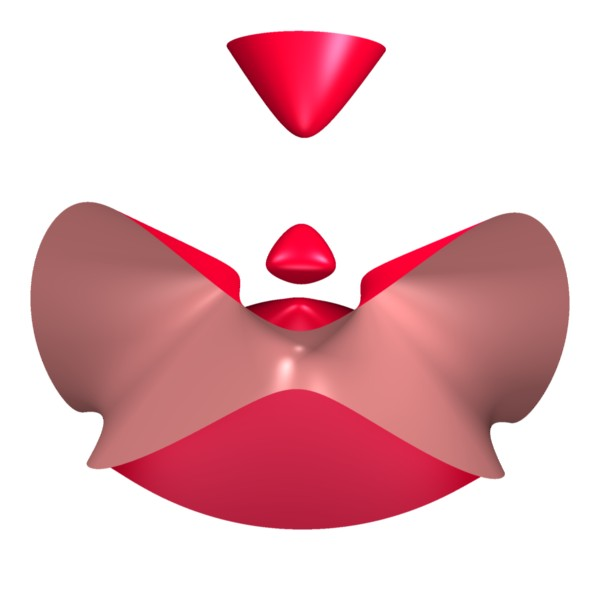
\includegraphics[width=1.35cm]{./../../common/images/cayley_cubic_3}
        \end{tabular}
      \end{tabular}
    \end{center}
\end{surferPage}
